\documentclass[11pt]{article}
\usepackage[a4paper, total={6in, 10in}]{geometry}
%\usepackage[hyphens]{url} % <-- new
\usepackage{natbib}

\usepackage{graphicx} %Loading the package
\graphicspath{{../src/sinewaves/}}


\usepackage{xspace}
\newcommand{\R}{\textsf{R}\xspace}

%% Codelinks
\usepackage{hyperref}
\usepackage{fontawesome}
\usepackage{color}
\definecolor{linkcolor}{rgb}{0.1216,0.4667,0.7059} % blue for ONLINE version
%%\definecolor{linkcolor}{rgb}{0.0, 0.0, 0.0} % black for PRINTER version
\newcommand{\codeicon}{{\color{linkcolor}\faFileCodeO}}
\newcommand{\codelink}[1]{\href{#1}{\codeicon}}


\author{Miguel Xochicale\\
%miguelpxochicale at gmail dot com\\
%School of Engineering\\
%Department of Electronic, Electric and System Engineering\\
}


\title{Surrogate Data Analysis} 

\date{30th August 2019}



\begin{document}
\maketitle


THE FOLLOWING PARAGRAPH IS AN EXTRACT FROM \\
"Chapter 7.2 Future Work: Surrogate Data Analysis" \\


Non-stationarity and non-linearity of experimental time-series data 
were assumed in this thesis (see Chapter 1).
Such assumption was made based on the ambiguity of 
nonlinear analysis methods to quantify movement variability
and the not yet fully explored area of application of nonlinear analysis 
methods in human-humanoid interaction (see Chapters 1 and 2). 
From the examiners of the PhD viva, 
one recommendation to avoid such prejudice of the type of data  
is to test the non-linearity and non-stationarity  
of the experimental time series data before nonlinear analysis 
methods are applied.
Hence, a possible avenue to tackle such caveat 
is to apply surrogate data analysis to test that 
data have not been generated by "a stationary Gaussian linear
stochastic process that is observed through an invertible,
static, but possible linear stochastic function" 
\citep[p. 2]{schreiber2000}.
However, applying surrogate data analysis to time series data 
that show strong periodicity or quasi-periodicity 
might create misleading results and perhaps provide unfair 
conclusion 
(see the following figures that illustrate how different 
realisations of the same periodic sinusoidal signal 
show to be sometimes stationarity and others non-stationarity).
Hence, further research require to be done,
perhaps consider the works of 
\cite{stam1998} and  \cite{small2002}
to test weak non-stationarity 
of periodic and quasi-periodic time series data.
Also, for future work, 
it can be considered other time series data from 
activities that involve more than one joint 
in order to test the robustness of 
not only nonlinear analysis methods but 
also surrogate data analysis.



%---------------------------------(FIGURE)-------------------------------------
\begin{figure}
\centering
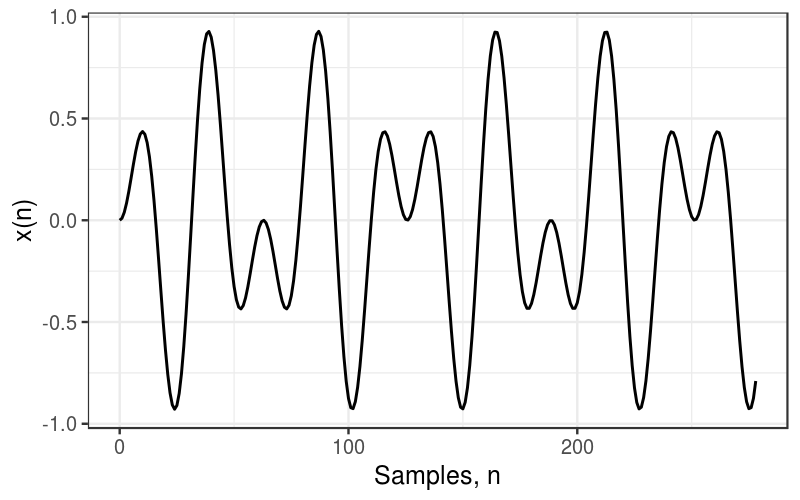
\includegraphics[width=0.6\textwidth]{r0_ts_sinewaves_window_length_278} %Importing a figure
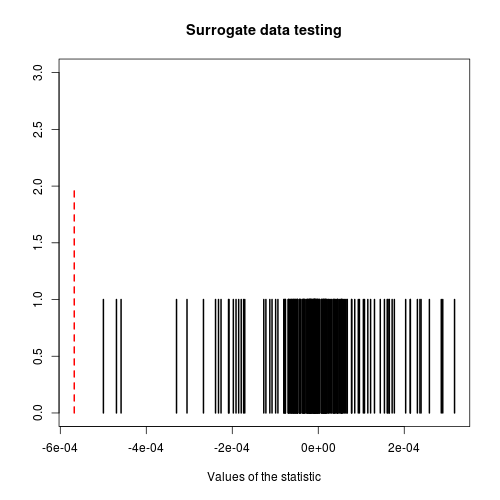
\includegraphics[width=0.6\textwidth]{r0_sdt_sinewaves_window_length_278} %Importing a figure
    \caption[]{
	{\bf Realisation 0.}
	(A) Sinewave time series and (B) surrogate data testing.
	\R code to reproduce the figure is available at 
	\codelink{https://github.com/mxochicale-phd/thesis/blob/master/0_code_data/1_code/x_surrogate/00_timeseries/code/B_.R}
	}
    \label{fig:thesis-outline}
\end{figure}
%%---------------------------------(FIGURE)-------------------------------------


%---------------------------------(FIGURE)-------------------------------------
\begin{figure}
\centering
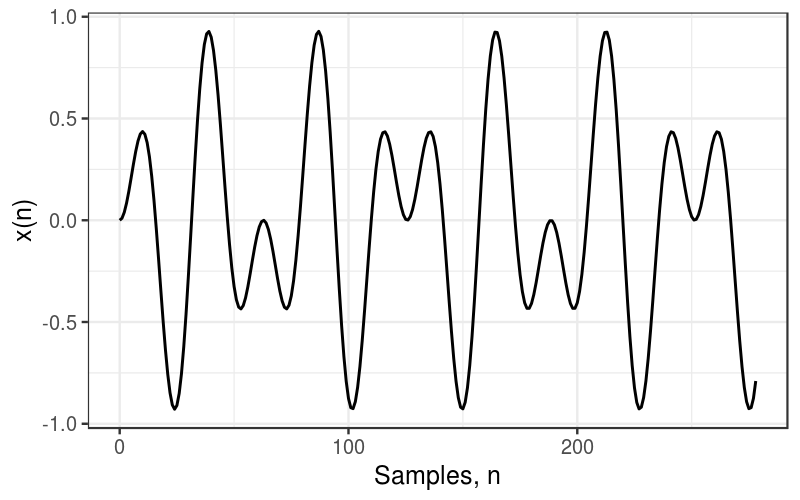
\includegraphics[width=0.6\textwidth]{r1_ts_sinewaves_window_length_278} %Importing a figure
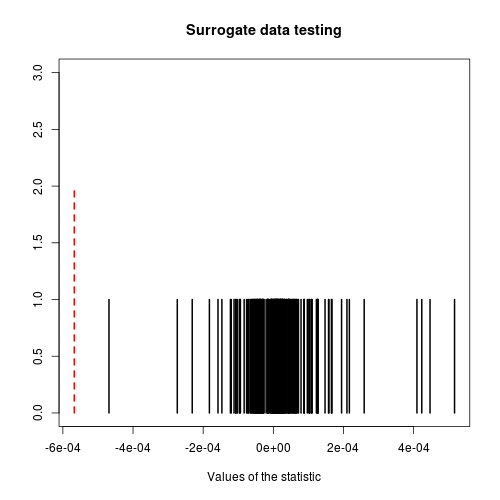
\includegraphics[width=0.6\textwidth]{r1_sdt_sinewaves_window_length_278} %Importing a figure
    \caption[]{
	{\bf Realisation 1.}
	(A) Sinewave time series and (B) surrogate data testing.
	\R code to reproduce the figure is available at 
	\codelink{https://github.com/mxochicale-phd/thesis/blob/master/0_code_data/1_code/x_surrogate/00_timeseries/code/B_.R}

}
    \label{fig:thesis-outline}
\end{figure}
%%---------------------------------(FIGURE)-------------------------------------




%---------------------------------(FIGURE)-------------------------------------
\begin{figure}
\centering
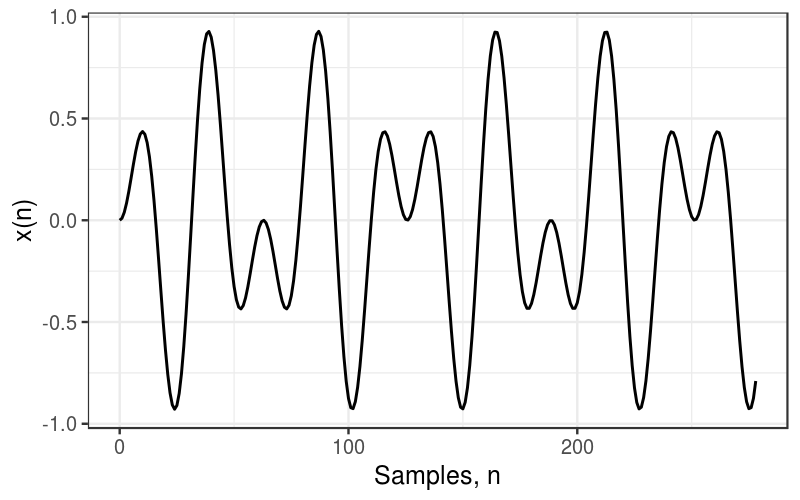
\includegraphics[width=0.6\textwidth]{r2_ts_sinewaves_window_length_278} %Importing a figure
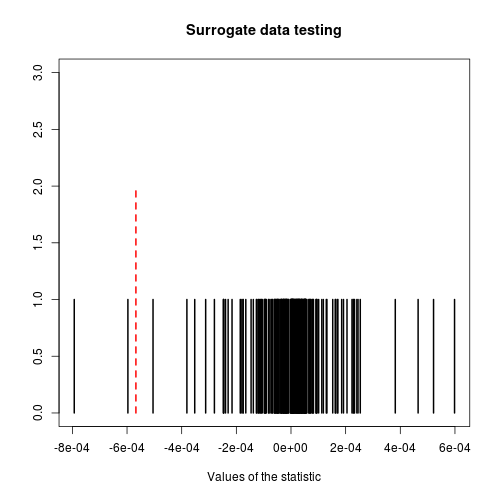
\includegraphics[width=0.6\textwidth]{r2_sdt_sinewaves_window_length_278} %Importing a figure
    \caption[]{
	{\bf Realisation 2.}
	(A) Sinewave time series and (B) surrogate data testing.
	\R code to reproduce the figure is available at 
	\codelink{https://github.com/mxochicale-phd/thesis/blob/master/0_code_data/1_code/x_surrogate/00_timeseries/code/B_.R}

}
    \label{fig:thesis-outline}
\end{figure}
%%---------------------------------(FIGURE)-------------------------------------




%---------------------------------(FIGURE)-------------------------------------
\begin{figure}
\centering
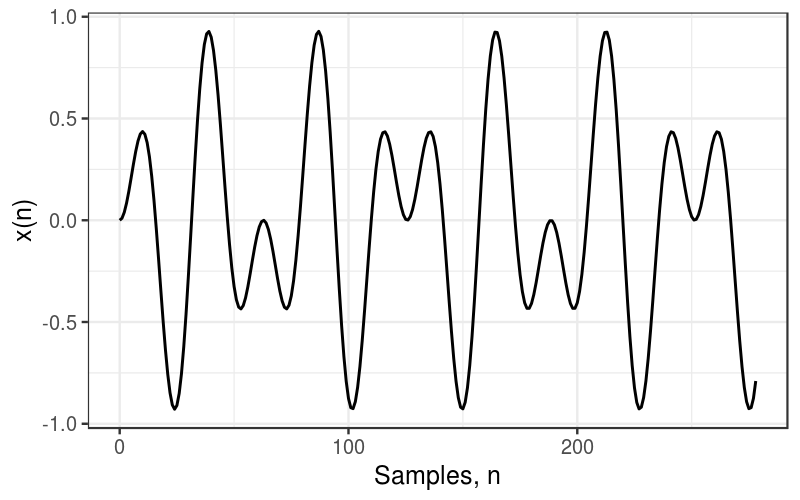
\includegraphics[width=0.6\textwidth]{r3_ts_sinewaves_window_length_278} %Importing a figure
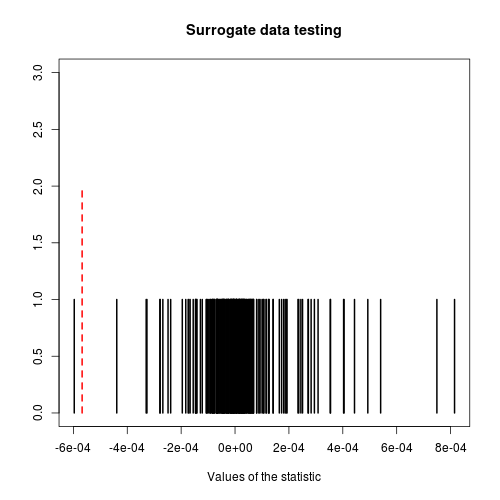
\includegraphics[width=0.6\textwidth]{r3_sdt_sinewaves_window_length_278} %Importing a figure
    \caption[]{
	{\bf Realisation 3.}
	(A) Sinewave time series and (B) surrogate data testing.
	\R code to reproduce the figure is available at 
	\codelink{https://github.com/mxochicale-phd/thesis/blob/master/0_code_data/1_code/x_surrogate/00_timeseries/code/B_.R}

}
    \label{fig:thesis-outline}
\end{figure}
%%---------------------------------(FIGURE)-------------------------------------






%---------------------------------(FIGURE)-------------------------------------
\begin{figure}
\centering
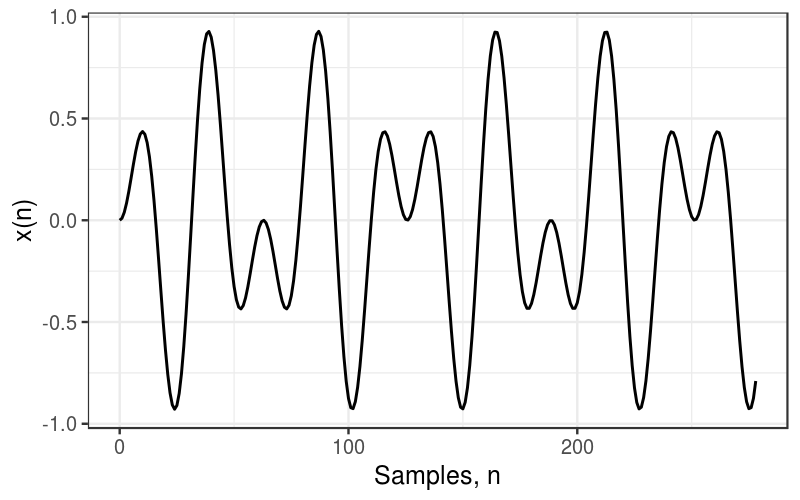
\includegraphics[width=0.6\textwidth]{r4_ts_sinewaves_window_length_278} %Importing a figure
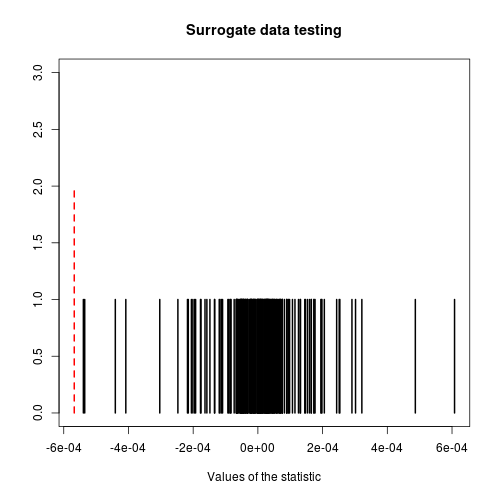
\includegraphics[width=0.6\textwidth]{r4_sdt_sinewaves_window_length_278} %Importing a figure
    \caption[]{
	{\bf Realisation 4.}
	(A) Sinewave time series and (B) surrogate data testing.
	\R code to reproduce the figure is available at 
	\codelink{https://github.com/mxochicale-phd/thesis/blob/master/0_code_data/1_code/x_surrogate/00_timeseries/code/B_.R}
}
    \label{fig:thesis-outline}
\end{figure}
%%---------------------------------(FIGURE)-------------------------------------









%---------------------------------(FIGURE)-------------------------------------
\begin{figure}
\centering
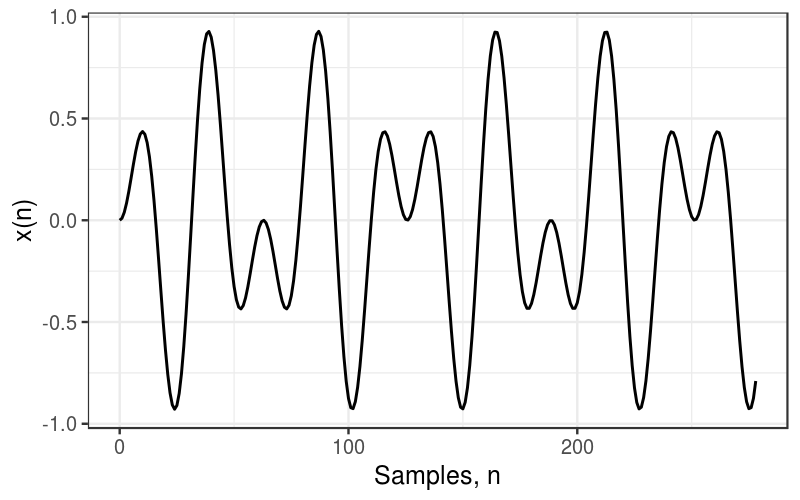
\includegraphics[width=0.6\textwidth]{r5_ts_sinewaves_window_length_278} %Importing a figure
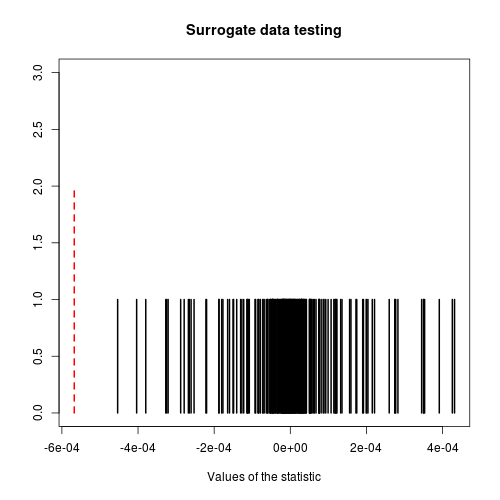
\includegraphics[width=0.6\textwidth]{r5_sdt_sinewaves_window_length_278} %Importing a figure
    \caption[]{
	{\bf Realisation 5.}
	(A) Sinewave time series and (B) surrogate data testing.
	\R code to reproduce the figure is available at 
	\codelink{https://github.com/mxochicale-phd/thesis/blob/master/0_code_data/1_code/x_surrogate/00_timeseries/code/B_.R}
}
    \label{fig:thesis-outline}
\end{figure}
%%---------------------------------(FIGURE)-------------------------------------







%---------------------------------(FIGURE)-------------------------------------
\begin{figure}
\centering
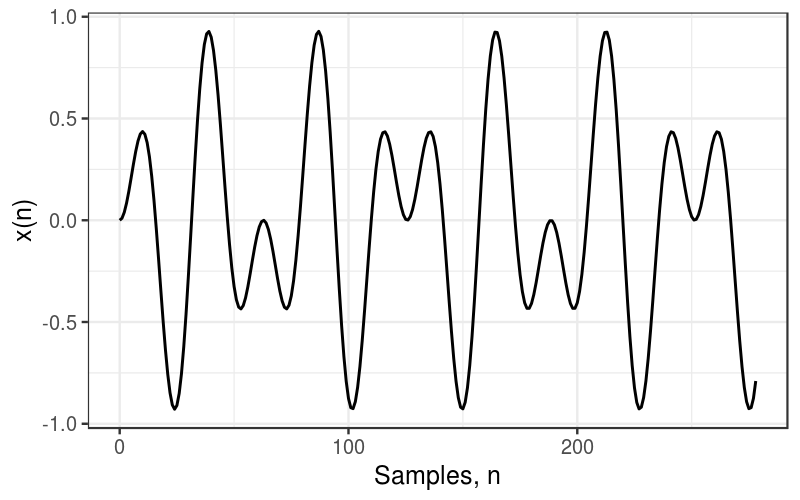
\includegraphics[width=0.6\textwidth]{r6_ts_sinewaves_window_length_278} %Importing a figure
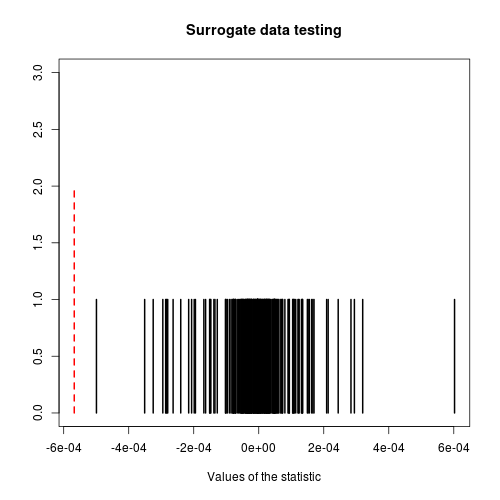
\includegraphics[width=0.6\textwidth]{r6_sdt_sinewaves_window_length_278} %Importing a figure
    \caption[]{
	{\bf Realisation 6.}
	(A) Sinewave time series and (B) surrogate data testing.
	\R code to reproduce the figure is available at 
	\codelink{https://github.com/mxochicale-phd/thesis/blob/master/0_code_data/1_code/x_surrogate/00_timeseries/code/B_.R}
	}
    \label{fig:thesis-outline}
\end{figure}
%%---------------------------------(FIGURE)-------------------------------------






%---------------------------------(FIGURE)-------------------------------------
\begin{figure}
\centering
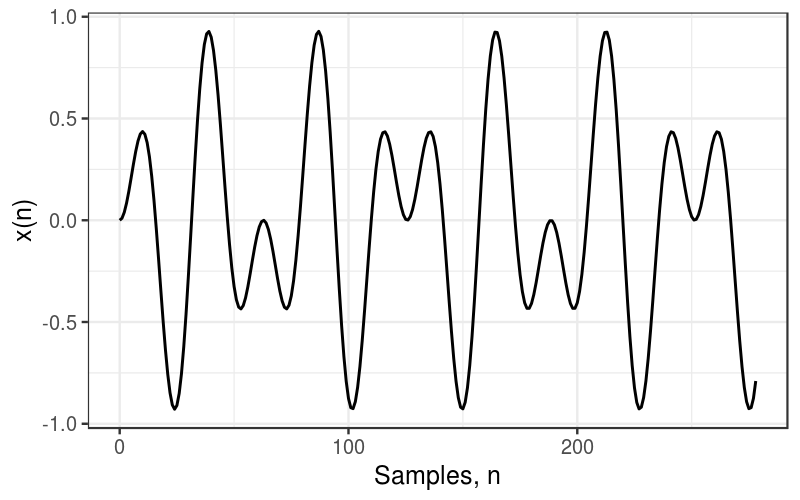
\includegraphics[width=0.6\textwidth]{r7_ts_sinewaves_window_length_278} %Importing a figure
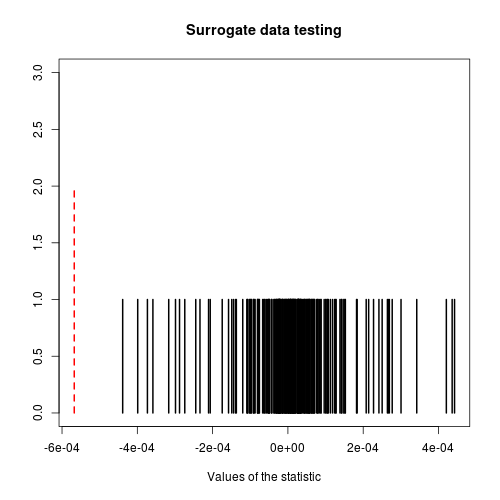
\includegraphics[width=0.6\textwidth]{r7_sdt_sinewaves_window_length_278} %Importing a figure
    \caption[]{
	{\bf Realisation 7.}
	(A) Sinewave time series and (B) surrogate data testing.
	\R code to reproduce the figure is available at 
	\codelink{https://github.com/mxochicale-phd/thesis/blob/master/0_code_data/1_code/x_surrogate/00_timeseries/code/B_.R}
	}
    \label{fig:thesis-outline}
\end{figure}
%%---------------------------------(FIGURE)-------------------------------------




%---------------------------------(FIGURE)-------------------------------------
\begin{figure}
\centering
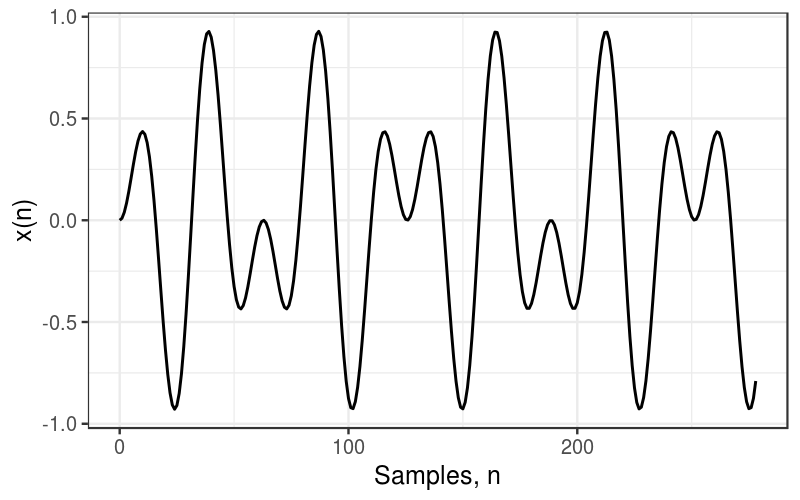
\includegraphics[width=0.6\textwidth]{r8_ts_sinewaves_window_length_278} %Importing a figure
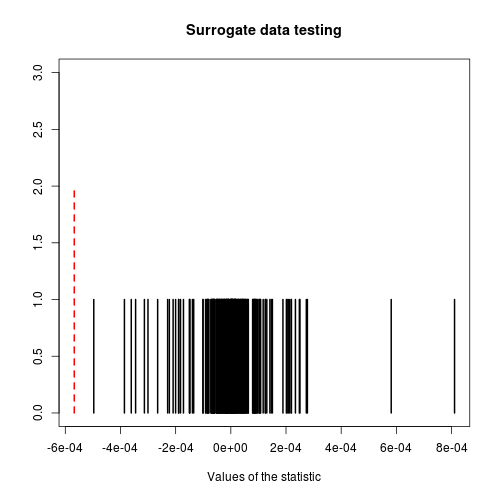
\includegraphics[width=0.6\textwidth]{r8_sdt_sinewaves_window_length_278} %Importing a figure
    \caption[]{
	{\bf Realisation 8.}
	(A) Sinewave time series and (B) surrogate data testing.
	\R code to reproduce the figure is available at 
	\codelink{https://github.com/mxochicale-phd/thesis/blob/master/0_code_data/1_code/x_surrogate/00_timeseries/code/B_.R}
	}
    \label{fig:thesis-outline}
\end{figure}
%%---------------------------------(FIGURE)-------------------------------------





%---------------------------------(FIGURE)-------------------------------------
\begin{figure}
\centering
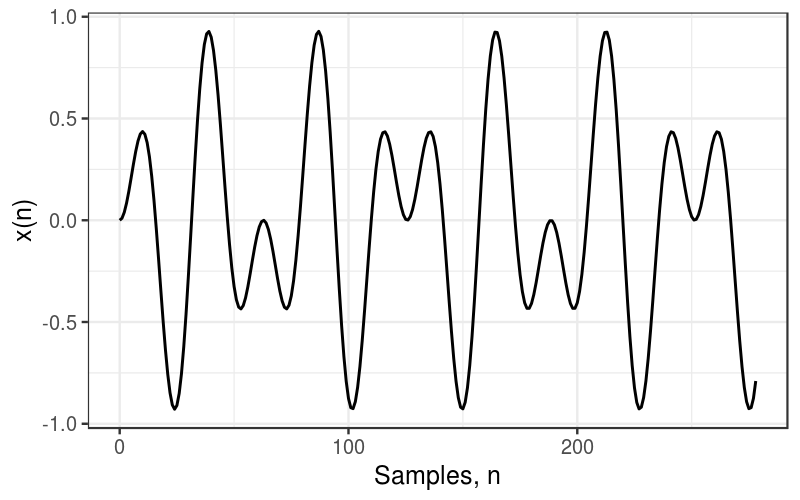
\includegraphics[width=0.6\textwidth]{r9_ts_sinewaves_window_length_278} %Importing a figure
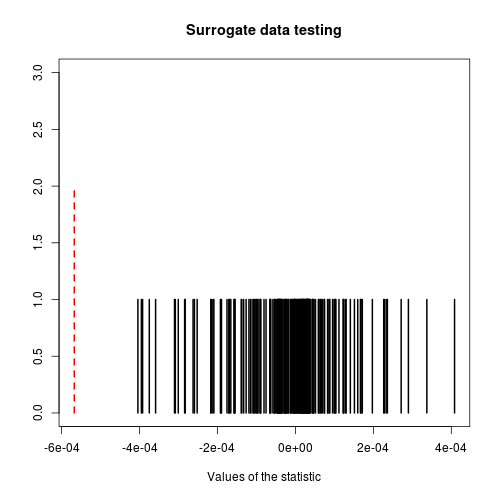
\includegraphics[width=0.6\textwidth]{r9_sdt_sinewaves_window_length_278} %Importing a figure
    \caption[]{
	{\bf Realisation 9.}
	(A) Sinewave time series and (B) surrogate data testing.
	\R code to reproduce the figure is available at 
	\codelink{https://github.com/mxochicale-phd/thesis/blob/master/0_code_data/1_code/x_surrogate/00_timeseries/code/B_.R}
	}
    \label{fig:thesis-outline}
\end{figure}
%%---------------------------------(FIGURE)-------------------------------------










\bibliography{references}
\bibliographystyle{apalike}

\end{document}
